\documentclass{standalone}
\begin{document}
	\subsection{Color Quantization for Image Segmentation}
	

	Color quantization is the process of reducing the number of colors in a digital image. The main objective of quantization process is that 
	significant information should be preserved while reducing the number of colors in an image, in other word quantization process shouldn’t cause 
	significant information loss in the image. 
	Color quantization, accepted as a pre-processing application, is used to reduce the number of colors in images with minimum distortion such that the 
	reproduced image should be very close to the original image visually, as in \figurename\,\ref{fig:ColorQuantization}. 

	\begin{figure}[hp]
		\label{fig:ColorQuantization}
		\centering
			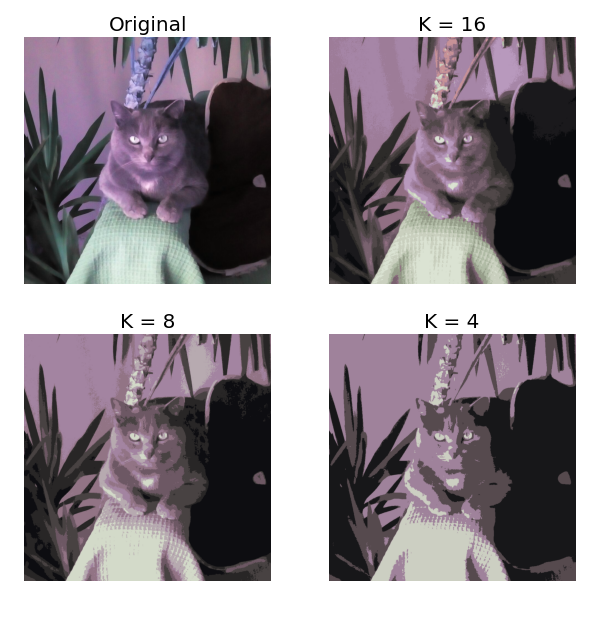
\includegraphics[scale=.5]{ColorQuantization.png}
		\caption{\textit{Color quantized RGB image. We observe the original image, a 16 color image which look similar to the original one, a 8 colors image and 4 colors image}}
	\end{figure}

	Color quantization play an important role in many filed of applications such as segmentation, compression, color texture analysis, watermarking, 
	text localization/detection, nonphotorealistic rendering and content-based retrieval~\cite{ART:Ozturk}.\\
	
	As I've said before I have used this technique to segment medical images by grouping each tissue by color similarity. The relation between the kind of tissue and the voxel color is given by  and the Hounsfield Units(HU) : Pixels colors are proportional to HU, which are defined as a linear transformation of the linear attenuation coefficient($\mu$). HU normalize the $\mu$ of a particular tissue according to a reference one, usually water($\mu_{H_2 O}$), ss we can see in equation\,\ref{eq:HU} : 
	
	\begin{equation}\label{eq:HU}
		HU = \frac{\mu - \mu_{H_2 O}}{\mu_{H_2 O}}
	\end{equation}
		
	In the end each color results proportional to the linear attenuation coefficient, different from each tissue, so exist a relation between the GL and the tissue type which is exploit by its intensity, that makes this techniques available. 

	
	
	Up to now we have discussed about single voxel intesnity, but its also possible to exploit informations about neighbouring pixels, by building a suitable color space: this is useful since lesions areas involves many closed voxels. 
	In digital image processing, images are represented with a 3D tensor, in which the first two dimensions represent the height and width of the image 
	and the last one the number of channels. Gray scale images requires only one channel, so each pixel has a numeric values whose range may change 
	according to the image format. On the other hand color images requires 3 channels, and the value of each channel represent the level of the primary 
	color stored in this particular channel, so each color is represented by 3 different values, according to Young theory. \\
	In our case we have decided to use more than 3 channels and each one of them incorporates different information like edges information or 
	neighbouring pixels information. In the end we have build a color space of several dimensions in which each color is represented by different image 
	features like edges and median neighbouring intensity. 
	
	To find the characteristic color of each tissue, which is a centroids in the color space, I've used a simple kmeans clustering, since it provides a suitable segmentation with good time performances, since it is efficiently implemented for multi-channel images in OpenCV. 
	Kmeans clustering requires a prior knowledge on the number of cluster, which in our case is given by the anatomical structure of the lung, so each cluster will correspond to a different anatomical structure: 
	\begin{itemize}
		\item Total lung parenchima
		\item Bronchial and vessels
		\item \textbf{GGO}
		\item Eventual noise
	\end{itemize}

	



	
	
	
	

	
	
\end{document}